\documentclass[finals,table,dvipsnames]{beamer}
\usefonttheme{professionalfonts}

\usepackage[english]{babel}
\usepackage[utf8]{inputenc}
\usepackage[T1]{fontenc}
\usepackage{amsmath}
\usepackage{multicol}
\usepackage{graphicx}
\usepackage{hyperref}
\usepackage{float}
\usepackage{url}
\usepackage{wasysym}
\usepackage{xspace}
\usepackage{times}
\usepackage{booktabs}
\usepackage{xcolor}
\usepackage{marvosym}
\usepackage{tikz}
\usepackage{listings}
\usepackage{fancybox}
\usepackage{shadow}


\usetikzlibrary{arrows,shapes,backgrounds}
\tikzstyle{every picture}+=[remember picture]
\tikzstyle{na} = [baseline=-.5ex]

\DeclareGraphicsExtensions{.eps,.pdf,.JPG,.jpg,.jpeg,.png,.PNG}
\graphicspath{
{./figures/}
}
\definecolor{sdnblue}{HTML}{005baa}
\definecolor{sdngrey}{HTML}{646464}

\setbeamertemplate{navigation symbols}{}
\setbeamercolor{title}{fg=sdnblue}
\setbeamertemplate{footline}[frame number]
%\setbeamercolor{background canvas}{bg=black!95}
%\setbeamercolor{normal text}{bg=black,fg=white}
\setbeamercolor{frametitle}{fg=sdnblue}
%\setbeamercolor{section in sidebar}{fg=blue!70}
%\setbeamercolor{sidebar}{fg=black}
%\setbeamercolor{structure}{bg=black,fg=black!5}
%\setbeamercolor{item projected}{fg=black,bg=white}


\setbeamertemplate{items}[square] 
\setbeamertemplate{caption}[numbered]
\setbeamerfont{caption}{size=\scriptsize,family=\it}
\usefonttheme{professionalfonts} % using non standard fonts for beamer
\usefonttheme{serif} % default family is serif

%--------------------------------
\hypersetup{bookmarksopen=true,
bookmarksnumbered=true,  
pdffitwindow=true, 
pdfstartview=Fit,
%pdfpagemode=FullScreen,
pdffitwindow=true,
pdftoolbar=true,
pdfmenubar=true,
pdfwindowui=true,
pdfauthor={Alexander Barth{,} Aida Alvera-Azc\'{a}rate{,} Mohamed~Ouberdous{,} Charles~Troupin{,} Sylvain~Watelet \& Jean-Marie~Beckers},
pdfsubject={DIVA Lecce 2016},
pdftitle={DIVA Lecce 2016},
bookmarksopenlevel=0,
colorlinks=true,
linkcolor=blue,anchorcolor=black,%
citecolor=blue,filecolor=black,%
menucolor=black,urlcolor=blue,%
pdfpageduration=1,%
pdffitwindow=true
}

\logo{\vspace{-5mm}
\includegraphics[height=0.5cm]{gherlogo_transparent}~
\includegraphics[height=0.5cm]{Logo_SeaDataNet_fond_transparent}\hspace{7mm}}

\author[Alexander Barth, Aida Alvera-Azc\'{a}rate, Mohamed~Ouberdous, Charles~Troupin, Sylvain~Watelet \& Jean-Marie~Beckers]{Alexander Barth, Aida Alvera-Azc\'{a}rate, Mohamed~Ouberdous,\\
 Charles~Troupin, Sylvain~Watelet \& Jean-Marie~Beckers}
  
\title[]{\diva Lecce 2016}
\date{Lecce (Italy), 11--14 April 2016}


%--------------------------------

\definecolor{colorcite}{rgb}{0,.46,.46}
\newcommand{\diva}{\textsf{Diva}\xspace}
\newcommand{\mat}{\mathbf}
\newcommand{\important}[1]{\textcolor{sdnblue}{#1}}
\newcommand{\method}[1]{\textcolor{gray}{#1}}
\newcommand{\tool}[1]{\textcolor{sdngrey}{\texttt{#1}}}
\newcommand{\nablab}{\boldsymbol{\nabla}}
\newcommand{\ddiff}{\mbox{d}}
\newcommand{\cita}[1]{\textcolor{colorcite}{#1}}
\newcommand{\fleche}{$\rightarrow$\,}
\newcommand{\snr}{\lambda}
\newcommand{\noise}{\epsilon}

\newcommand{\directory}[1]{\texttt{\color{ForestGreen}{#1}}}
\newcommand{\file}[1]{\texttt{\color{MidnightBlue}{#1}}}
\newcommand{\command}[1]{\texttt{\color{RedOrange}{#1}}}
\newcommand{\resfile}[1]{\texttt{\color{MidnightBlue}{#1}}}

\newcommand{\statmean}[1]{\left\langle #1 \right\rangle}
\newcommand{\true}[1]{{#1}^t}
\newcommand{\analyzed}[1]{{#1}^a}
\newcommand{\observation}{ \mbox{\boldmath   $ \protect\mathrm{y} $} }
\newcommand{\forecasted}[1]{{#1}^f}
\newcommand{\kalmangain}{\matr{K}}
\newcommand{\Hobs}{\matr{H}}
\newcommand{\errorv}{\vect{\epsilon}}
\newcommand{\errorobs}{\vect{\epsilon}^o}
\newcommand{\Perr}{\matr{P}}
\newcommand{\Rerr}{\matr{R}}

\newcommand{\matr}[1] { \mbox{\boldmath   $ \protect\mathsf{#1} $} }
\newcommand{\trcon}[1]{{#1}^\star}
\newcommand{\adj}[1]{\trcon{#1}}
\newcommand{\elem}[2]{\left( #1 \right)_{#2}}
\newcommand{\trace}{\operatorname{trace}}
\newcommand{\sing}{\rho}

\newcommand{\myshadowbox}[1]{\shabox{\parbox{10cm}{#1}}}
\newcommand{\inv}[1]{{#1}^{ \mbox{\small{-}}  1}}

\lstdefinestyle{Bash}
{language=bash,
keywordstyle=\color{blue},
basicstyle=\ttfamily,
morekeywords={ctroupin@gher13},
alsoletter={:~$},
commentstyle=\color{dkgreen},
morekeywords=[2]{ctroupin@gher13:},
keywordstyle=[2]{\color{red}},
literate={\$}{{\textcolor{red}{\$}}}1 
         {:}{{\textcolor{red}{:}}}1
         {~}{{\textcolor{red}{\textasciitilde}}}1,
}
\lstset{
    breaklines     = true,
    frame          = single,
    rulecolor=     \color{gray},
}

%$

%-------------------------------------------------------------------------
\newcommand{\maketitlepage}{{
\usebackgroundtemplate{\hspace{-1cm}\tikz\node[opacity=0.2]{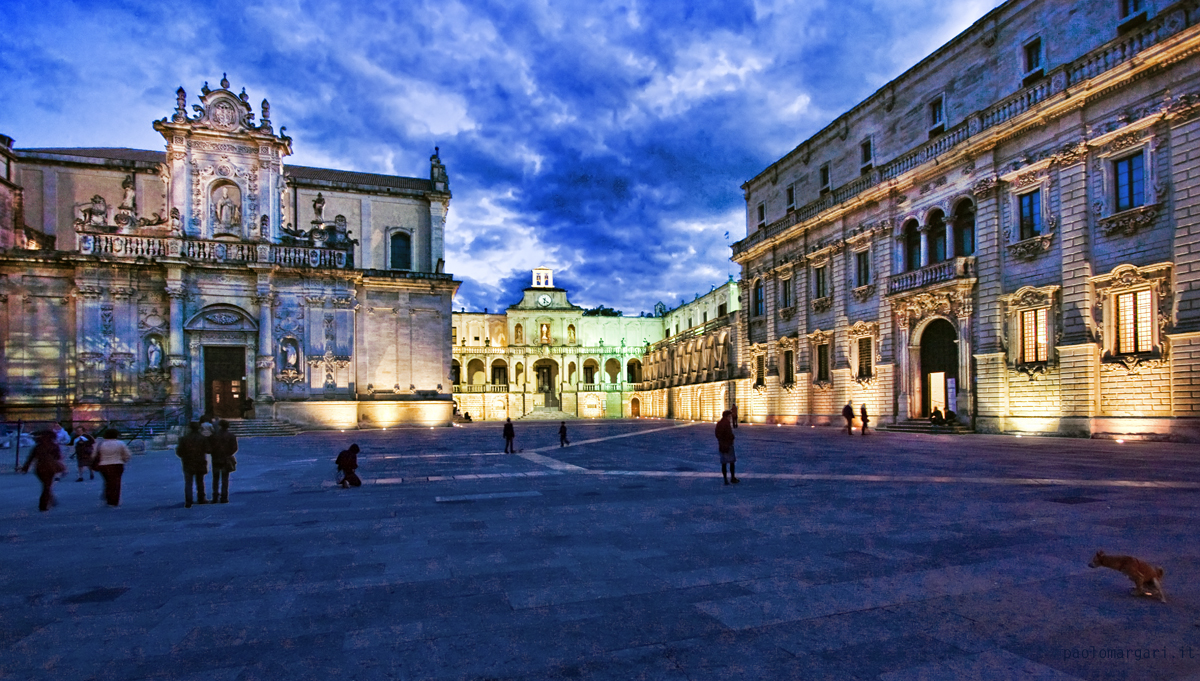
\includegraphics[height=1.05\paperheight]{Lecce1.jpg}};}
\begin{frame}
\centering
\footnotesize
\maketitle
\vspace{-.25cm}
\tiny{\textbf{Acknowledgements:} SeaDataNet, EMODnet Chemistry, \\
EMODnet Biology, STARESO}
\vspace{.125cm}

\begin{figure}
\centering

\includegraphics[width=.1\paperwidth]{gherlogo_transparent.PNG}\hspace*{.5cm}
\includegraphics[width=.1\paperwidth]{logo_ulg}\hspace*{.5cm}
\includegraphics[width=.1\paperwidth]{Logo_SeaDataNet_fond_transparent}\hspace*{.5cm}
\includegraphics[width=.07\paperwidth]{logo_emodnet}\hspace*{.5cm}
\includegraphics[width=.09\paperwidth]{Logo_Stareso}
\end{figure}

\end{frame}
}}
%-------------------------------------------------------------------------

\parindent 0cm

\author[Alexander Barth, Aida Alvera-Azc\'{a}rate, Mohamed~Ouberdous, ctroupin~Troupin, Sylvain~Watelet \& Jean-Marie~Beckers]{Alexander Barth, Aida Alvera-Azc\'{a}rate, Mohamed~Ouberdous,\\
 ctroupin~Troupin, Sylvain~Watelet \& Jean-Marie~Beckers}
  
\title[]{\diva Lecce 2016}
\subtitle{Installation and tests}
\date{}
\begin{document}

\maketitlepage % defined in GHERheader2013.tex

%--------------------------------------------------------------------------------------------------------
\begin{frame}[fragile]
\frametitle{Download and extract the code}
\footnotesize

Create directory and download \diva archive 
\begin{lstlisting}[style=Bash]
[swatelet@gher ~]$ mkdir DIVA
[swatelet@gher ~]$ cd DIVA/
[swatelet@gher DIVA]$ wget http://modb.oce.ulg.ac.be/mediawiki/upload/DIVA/releases/diva-4.6.11.tgz
\end{lstlisting}

Extract the archive and go in the main directory:
\begin{lstlisting}[style=Bash]
[swatelet@gher DIVA]$ tar -xzf diva-4.6.11.tgz
[swatelet@gher DIVA]$ cd diva-4.6.11/
\end{lstlisting}
If you already have a running older version, retrieve your \file{divacompile\_options} and put it in place of the default in DIVA3D/src/Fortran/
\end{frame}

%--------------------------------------------------------------------------------------------------------
\begin{frame}[fragile]
\frametitle{Compilation}
\footnotesize

Go to source directory
\begin{lstlisting}[style=Bash]
swatelet@gher ~/DIVA/diva-4.6.11 $ cd DIVA3D/src/Fortran/
\end{lstlisting}

Run divacompilall \Coffeecup
\begin{lstlisting}[style=Bash]
swatelet@gher ~/DIVA/diva-4.6.11/DIVA3D/src/Fortran $ ./divacompileall
\end{lstlisting}

You should get:\\
\begin{verbatim}
You have compiled 112 programs
out of 112
Writing log file...
--> written in compilation.log
...
\end{verbatim}

Otherwise: edit \file{divacompile\_options}

\end{frame}

\begin{frame}
\frametitle{Alternative installation: virtual box}
\begin{itemize}
\item Image \file{DIVA\_Clone.tgz} on USB stick (Sylvain)
\item Installation description \url{http://modb.oce.ulg.ac.be/mediawiki/upload/DIVA/notes/virtualbox.pdf}
\end{itemize}

\begin{enumerate}
\item Installation of virtualbox (4.3.12 or later)
\item Extract virtual machine \file{DIVA\_Clone/vdi} (time consuming unzip)
\item Configuration of VirtualBox (New, Name : DIVA, Type : Linux Ubuntu 32, select 2500 Mb RAM, search existing hard drive to locate \file{DIVA\_CLONE.vdi} and create virtual machine)
\item Ready to run tests as divauser with pw divauser in a terminal of the DIVA virtual machine
\end{enumerate}



\end{frame}
%--------------------------------------------------------------------------------------------------------
\begin{frame}[fragile]
\frametitle{Mandatory softwares}

\begin{enumerate}
\item bc
\item dos2unix
\end{enumerate}

for ubuntu-like OS :

\begin{lstlisting}[style=Bash]
swatelet@gher ~/DIVA/diva-4.6.11 $ sudo apt-get install bc
\end{lstlisting}

\begin{lstlisting}[style=Bash]
swatelet@gher ~/DIVA/diva-4.6.11 $ sudo apt-get install dos2unix
\end{lstlisting}

for cygwin :

\begin{lstlisting}[style=Bash]
swatelet@gher ~ $ lynx -source rawgit.com/transcode-open/apt-cyg/master/apt-cyg > apt-cyg
swatelet@gher ~ $ chmod +x apt-cyg
swatelet@gher ~ $ mv apt-cyg /usr/local/bin/
swatelet@gher ~ $ apt-cyg install bc
swatelet@gher ~ $ apt-cyg install dos2unix
\end{lstlisting}

source : \url{http://superuser.com/questions/41093/installing-cygwin-packages-from-the-command-line}

\end{frame}
%--------------------------------------------------------------------------------------------------------
\begin{frame}[fragile]
\frametitle{Configuration of the PATH}

In order to run diva correctly, you need to adapth your PATH variable.

\begin{lstlisting}[style=Bash]
swatelet@gher ~ $ ge .bashrc
\end{lstlisting}

then add these lines :

{\tiny
\begin{verbatim}
# personal PATH
PATH="$PATH:."
PATH="$PATH:/home/sylvain/DIVA/diva-4.6.11/DIVA3D/divastripped"
\end{verbatim}
}

\end{frame}
%--------------------------------------------------------------------------------------------------------

\begin{frame}[fragile]
\frametitle{Tests: 2D}
\footnotesize

Go to directory \directory{divastripped} (main directory for 2D runs)
\begin{lstlisting}[style=Bash]
swatelet@gher ~/DIVA/diva-4.6.11/DIVA3D/src/Fortran $ cd ../../divastripped/
\end{lstlisting}

Run \command{divatest0} \Coffeecup
\begin{lstlisting}[style=Bash]
swatelet@gher ~/DIVA/diva-4.6.11/DIVA3D/divastripped $ ./divatest0
\end{lstlisting}

\begin{columns}[totalwidth=\textwidth]
\column{.5\textwidth}
You should get:

{\tiny
\begin{verbatim}
Check the results in
./ouput/ghertonetcdf/results.nc (netcdf)
 
Field value at origin =  0.49961258873206416
\end{verbatim}
}
With ncview:
\column{.5\textwidth}

\begin{figure}
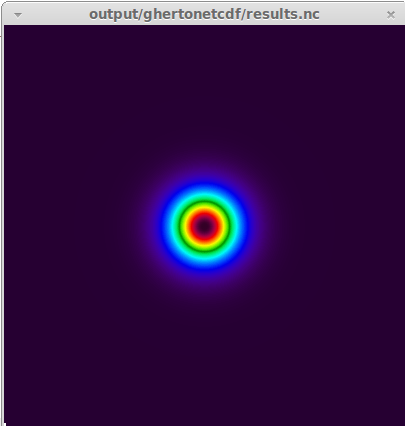
\includegraphics[width=.7\columnwidth]{divatest0_ncview}
\end{figure}

\end{columns}

\end{frame}

%--------------------------------------------------------------------------------------------------------
\begin{frame}[fragile]
\frametitle{Tests: 2D}
\footnotesize

Run \command{divatest}\hfill (test for pipes) \Coffeecup
\begin{lstlisting}[style=Bash]
swatelet@gher ~/DIVA/diva-4.6.11/DIVA3D/divastripped $ ./divatest
\end{lstlisting}

\begin{columns}[totalwidth=\textwidth]
\column{.5\textwidth}
If you get:

{\tiny
\begin{verbatim}
!!!!!!!!!!!!!!!!!!!!!!!!!!!!!!!!!!!!!!!!!!!!!!!
 Pipe does not work
 !!!!!!!!!!!!!!!!!!!!!!!!!!!!!!!!!!!!!!!!!!!!!!!
\end{verbatim}
}
then follow instructions on screen
\column{.5\textwidth}

\begin{figure}
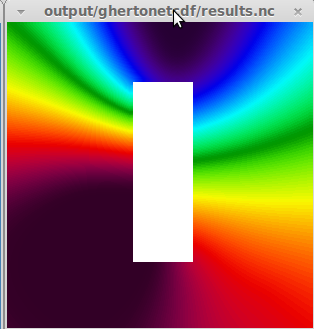
\includegraphics[width=.7\columnwidth]{divatest_ncview}
\end{figure}

\end{columns}
\end{frame}

%--------------------------------------------------------------------------------------------------------
\begin{frame}[fragile]
\frametitle{Tests: 2D}
\footnotesize

Run \command{divabigtest}\hfill (test for large data files) \Coffeecup\Coffeecup\Coffeecup
\begin{lstlisting}[style=Bash]
swatelet@gher ~/DIVA/diva-4.6.11/DIVA3D/divastripped $ ./divabigtest 100000
\end{lstlisting}

\begin{columns}[totalwidth=\textwidth]
\column{.5\textwidth}
You should get:

{\tiny
\begin{verbatim}
...
Check the results in
./ouput/ghertonetcdf/results.nc (netcdf)
Time for mesh creation:   0.830351  s
Time for calculation:     87.1226  s
Total time for analysis:  87.953  s
\end{verbatim}
}
otherwise: decrease number of data
\column{.5\textwidth}

\begin{figure}
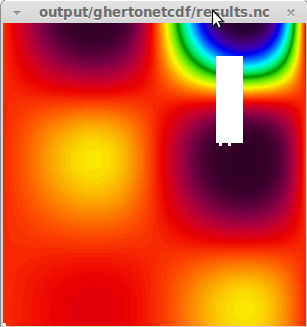
\includegraphics[width=.7\columnwidth]{divabigtest_ncview}
\end{figure}

\end{columns}
\end{frame}

%--------------------------------------------------------------------------------------------------------
\begin{frame}[fragile]
\frametitle{Tests: 4D}
\footnotesize
Go to directory \directory{Climatology} (main directory for 4D runs)
\begin{lstlisting}[style=Bash]
swatelet@gher ~/DIVA/diva-4.6.11/DIVA3D/divastripped $ cd ../../JRA4/Climatology/
\end{lstlisting}
Copy the input files from the \directory{Example4D}
\begin{lstlisting}[style=Bash]
swatelet@gher ~/DIVA/diva-4.6.11/JRA4/Climatology $ cp -r ../../Example4D/* .
\end{lstlisting}
Run \command{divadoall} \Coffeecup\Coffeecup
\begin{lstlisting}[style=Bash]
swatelet@gher ~/DIVA/diva-4.6.11/JRA4/Climatology $ ./divadoall > runtest.log
\end{lstlisting}

\begin{columns}[totalwidth=\textwidth]
\column{.4\textwidth}
You should get:
{\tiny
\begin{verbatim}
...
check-list of errors :
no error, you are lucky
divadoall: ==================
divadoall: Finished  Salinity
divadoall: ==================

\end{verbatim}
and results in \directory{output/3Danalysis/}
}
\column{.6\textwidth}

\begin{figure}
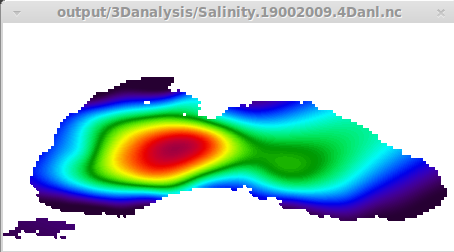
\includegraphics[width=.8\columnwidth]{divadoall_test_4D}
\end{figure}
\end{columns}

\end{frame}

\begin{frame}
\frametitle{Alternative installation in a virtual box}

Some optimisations can be used as explained in \url{http://www.howtogeek.com/124796/the-htg-guide-to-speeding-up-your-virtual-machines/}

\begin{itemize}
\item You might need to activate hardware virtualisation in your BIOS and then get access to multiprocessors
\item 3D video acceleration activation can also increase performance
\end{itemize}

Then you need to find a way to share files with your host machine: done for you already via
a shared folder called \file{Divaexchange\_guest} which is mounted automatically. Before launching th virtual machine, create a shared folder in your host machine, called \file{Divaexchange\_host} in your home directory.


\end{frame}

\end{document}
